\section{Semaine du 07/05/24 au 14/05/24}
\insertsectionframe
\subsection{Brendan}
\insertsubsectionframe

{
\smallframetitle
\subsubsection{Affichages}
\begin{frame}{Affichage des données sur une carte}
    \begin{block}{Détail}
        \begin{itemize}
            \item Découverte d'une bibliothèque d'affichage de données géographiques interactive : \texttt{Folium} ;
            \item Affichage des données et colorisation selon plusieurs critères : technologies (2G, 3G, \dots) ou opérateurs (Free, SFR, Bouygues Telecom ou Orange).
        \end{itemize}
    \end{block}

    \begin{alertblock}{Problème}
        Le nombre de données à afficher est très important et rend la visualisation très saccadée.
    \end{alertblock}

    \begin{block}{Solution}
        Afficher seulement une partie des données à la fois selon différent critères de sélection : par opérateurs, technologie ou région.
    \end{block}
\end{frame}



\begin{frame}{}
    \begin{figure}
        \includegraphics[width=0.7\textwidth]{images/France-Opérateurs.png}
        \caption{\label{fig:fr-op}Les opérateurs dans toute la France}
    \end{figure}
\end{frame}

\begin{frame}{}
    \begin{figure}
        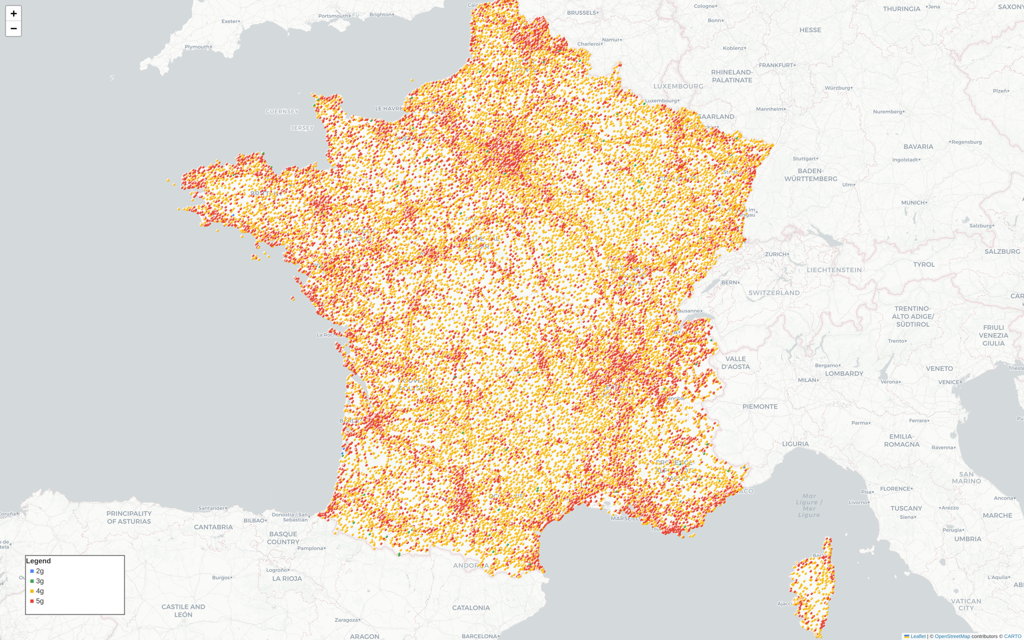
\includegraphics[width=0.7\textwidth]{images/France-Technologies.png}
        \caption{\label{fig:fr-tech}Les technologies dans toute la France}
    \end{figure}
\end{frame}

\begin{frame}{}
    \begin{figure}
        \includegraphics[width=0.7\textwidth]{images/Normandie-Opérateurs.png}
        \caption{\label{fig:no-op}Les opérateurs en Normandie}
    \end{figure}
\end{frame}

\begin{frame}{}
    \begin{figure}
        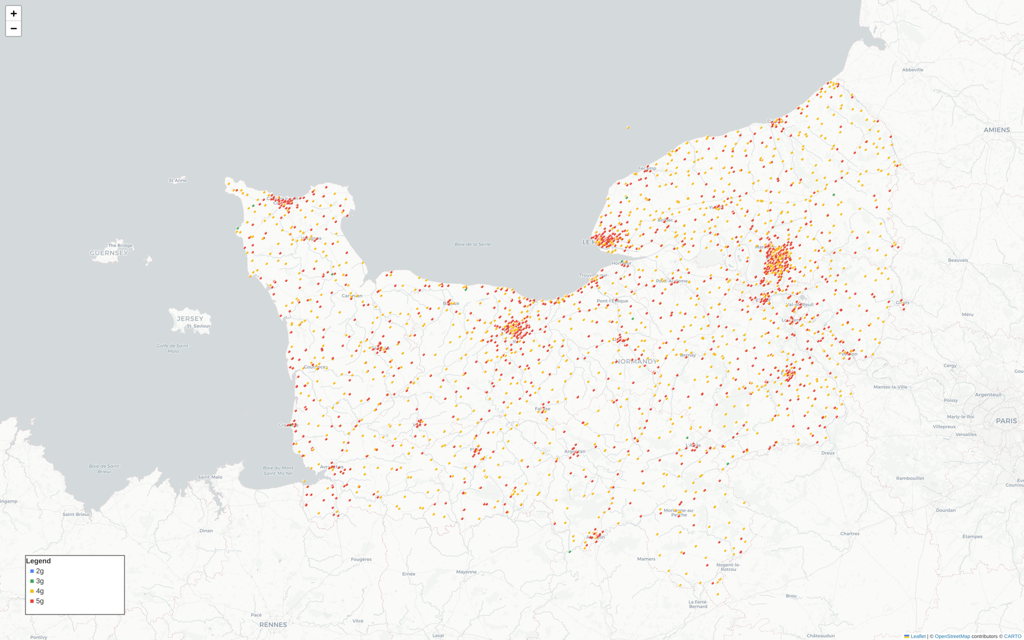
\includegraphics[width=0.7\textwidth]{images/Normandie-Technologies.png}
        \caption{\label{fig:no-tech}Les technologies en Normandie}
    \end{figure}
\end{frame}

\subsubsection{DBScan}
\begin{frame}{Détection des villes}
    Il est très clair que les stations de bases sont très regroupé au sein des villes. Il semble donc qu'il soit possible de détecter si les stations de bases sont en zone rurale ou urbaine à l'aide de la densité de stations de base

    \begin{block}{DBscan (1996)}
        L'algorithme DBscan (Density-Based spatial clustering of applications with noise) est un algorithme qui s'appuie sur la densité estimée des clusters pour effectuer le partitionnement.
    \end{block}
    \begin{block}{Paramètres}
        \begin{itemize}
            \item $\varepsilon$ : dissimilarité maximum entre deux individus ;
            \item $n_{\min}$ : cardinal minimum de chaque classe.
        \end{itemize}
    \end{block}
\end{frame}

\begin{frame}{Théorie : l'algorithme}
    \begin{block}{}
        \begin{enumerate}
            \item Pour chaque point $p_{j}$ :
                \begin{align*}
                    N\left(p_{i}\right) & \gets\left\{ p_{j}, j\in N=\left\{ 1, \dots, n\right\} \mid d(i,j)\leqslant\varepsilon\right\} \\
                    C & \gets\left\{ p_{i}\mid\left|N\left(p_{i}\right)\right|\geqslant n_{\min}\right\} 
                \end{align*}
            \item Construire le graphe de voisinage $G=\left(X, U\right)$, avec $$X=\left\{ p_{i}\mid i\in N\right\} \text{ et } U=\left\{ ij\mid i, j\in N,d(i,j)\leqslant\varepsilon\right\}$$
            \item Trouver les composantes connexes des sommets de $G$ (notées $G_{1}, \dots, G_{p}$) ;
            \item Pour chaque $p_{i}\notin C$ :
                \begin{align*}
                    j^{*} & =\arg\min_{1, \dots, p}\left(d\left(p_{i}, C_{k}\right)\right)\\
                    \text{si } & d\left(p_{i}, C_{j^{*}}\right)\leqslant\varepsilon\text{ alors}\\
                     & C_{j^{*}}\gets C_{j^{*}}\cup\left\{ p_{i}\right\} 
                \end{align*}
        \end{enumerate}
    \end{block}    
\end{frame}

\begin{frame}{}
    \begin{figure}
        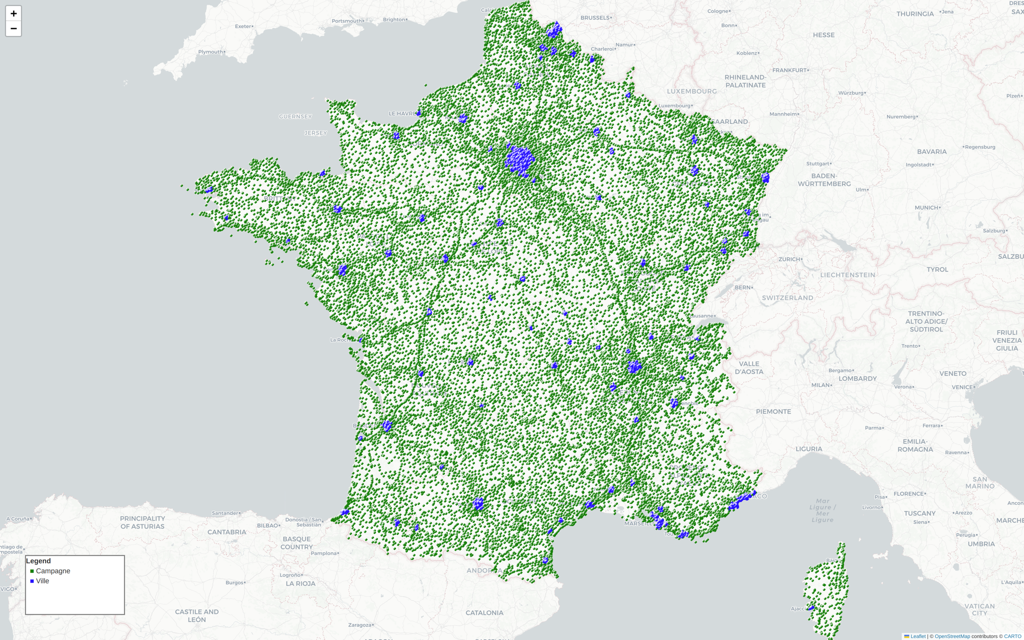
\includegraphics[width=0.7\textwidth]{images/France-Villes-Orange_0.03_15.png}
        \caption{\label{fig:fr-vi-or-0.03-15}Les villes détectées en France pour l'opérateur Orange avec $\epsilon=0.03$ et $n_{min}=15$}
    \end{figure}
\end{frame}


\subsubsection{Delaunay et Voronoï}

\begin{frame}{Diagramme de Voronoï}
    \begin{columns}
        \begin{column}{0.6\textwidth}
            \begin{block}{Définition}
                Le diagramme de Voronoï associé à un ensemble de points $(d_i)_{1\leq i \leq n}$ est un pavage de l'espace tel que chaque pavé $P_i$ représente l'ensemble des points plus proches de $d_i$ que de n'importe quel $d_j$ avec $j\neq i$ i.e.
            \end{block}
        \end{column}
            
        \begin{column}{0.4\textwidth}
            \begin{figure}
                
\includegraphics[width=0.5\textwidth]{images/Coloured_Voronoi_2D.png}
                \caption{\label{fig:vor-ex}Exemple de diagramme de Voronoï}
            \end{figure}
        \end{column}
    \end{columns}
    
            
\end{frame}

\begin{frame}{Triangulation de Delaunay}
    \begin{columns}
        \begin{column}{0.6\textwidth}
            \begin{block}{Définition}
                La triangulation de Delaunay d'un ensemble $P$ de points du plan est une triangulation $DT(P)$ telle qu'aucun point de $P$ n'est à l'intérieur du cercle circonscrit d'un des triangles de $DT(P)$. Les triangulations de Delaunay maximisent le plus petit angle de l'ensemble des angles des triangles, évitant ainsi les triangles \og allongés \fg{}.
            \end{block}
        \end{column}
            
        \begin{column}{0.4\textwidth}
             \begin{figure}
                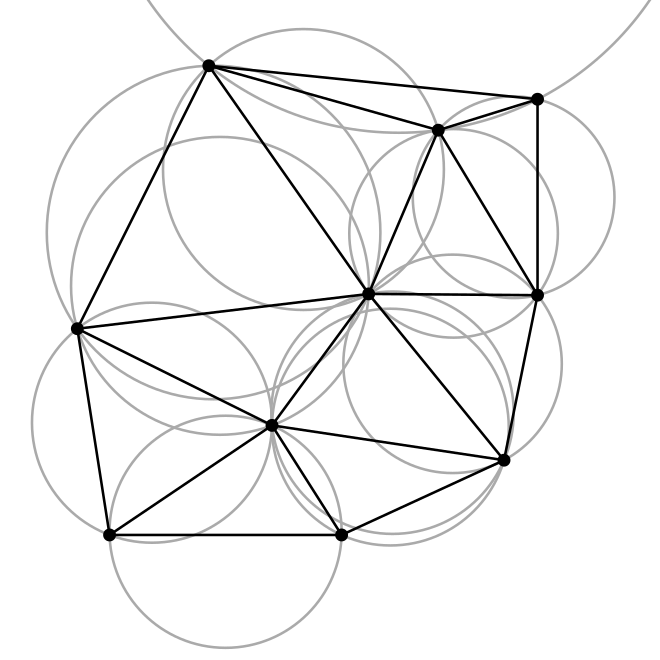
\includegraphics[width=0.5\textwidth]{images/Delaunay_circumcircles_vectorial.svg.png}
                \caption{\label{fig:del-ex}Exemple de triangulation de Delaunay}
            \end{figure}
        \end{column}
    \end{columns}
\end{frame}

\begin{frame}{Lien entre les 2}
    \begin{columns}
        \begin{column}{0.6\textwidth}
            \begin{block}{Propriétés}
                \begin{itemize}
                    \item La triangulation de Delaunay d’un ensemble discret $P$ de points est le graphe dual du diagramme de Voronoï associé à $P$;
                    \item Il est donc très facile de passer de l'un à l'autre (en temps polynomial);
                    \item il existe des algorithmes pour trouver une triangulation de Delaunay en $O(n\log(n))$.
                \end{itemize}      
            \end{block} 
        \end{column}
            
        \begin{column}{0.4\textwidth}
            \begin{figure}
                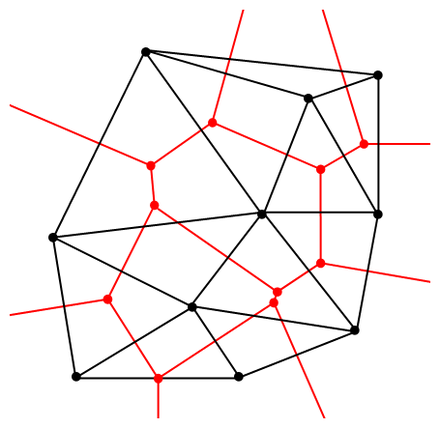
\includegraphics[width=0.5\textwidth]{images/Delaunay_Voronoi.png}
                \caption{\label{fig:del-vor}Lien entre Delaunay et Voronoï}
            \end{figure}
        \end{column}
    \end{columns} 
\end{frame}

\begin{frame}{Retour au problème}
    \begin{block}{Application à notre cas d'étude}
        Nous allons pouvoir utiliser ces notions en définissant :
        \begin{itemize}
            \item les voisins potentiels comme étant les triangles adjacents dans la triangulation de Delaunay
            \item les zones de couverture des antennes comme les pavés associé dans le diagramme de Voronoï
        \end{itemize}
    \end{block}
\end{frame}
}

\subsection{Paul}
\insertsubsectionframe

\begin{frame}{Résumé des épisodes précédents}
    Mon travail, pour la semaine qui vient de s'écouler, s'articule autour de trois axes majeurs :
    \begin{block}{}
        \begin{itemize}
            \item Découverte des données ;
            \item Documentation ;
            \item Reprise du travail de l'année précédente.
        \end{itemize}
    \end{block}
        
\end{frame}

{
\smallframetitle
\begin{frame}{Documentation}
    La majeure partie du travail de la semaine écoulée a consisté à se former aux différents outils de \texttt{Python} afin de pouvoir effectuer sereinement le travail.

    \begin{block}{Outils utilisés}
        \begin{itemize}
            \item \texttt{pandas.DataFrame} : gestion des données ;
            \item \texttt{scipy.spatial.Delaunay} : création de la triangulation de Delaunay ;
            \item \texttt{networkx.Graph} : création de graphes ;
            \item \texttt{matplotlib.pyplot} : affichage des résultats.
        \end{itemize}
    \end{block}
\end{frame}

\begin{frame}{Reprise du travail précédent (1/3)}
    La première tâche consistait à essayer de faire fonctionner le code fourni. Résultat : il ne fonctionne pas\dots
    
    Décision : refaire par moi-même. Cependant, j'ai gardé les idées.
    \begin{block}{Approche pour déterminer les voisins de stations de base}
        \begin{itemize}
            \item Faire une triangulation de Delaunay (liste de voisins potentiels);
            \item Eliminer les voisins distants de plus de $\unit[15]{km}$ ;
            \item Garder le voisin le plus proche dans chaque cadrant autour de chaque station (6 cadrants);
            \item Garder le voisin le plus proche quand deux stations voisines sont séparées par un angle faible.
        \end{itemize}
            
    \end{block}
\end{frame}

\begin{frame}{Reprise du travail précédent (2/3)}
    Ayant refait l'implantation moi-même, j'ai décidé d'utiliser les graphes au lieu de simplement les datasFrames : permettra de faciliter l'application de la théorie des graphes.
    \begin{block}{Apports de cette nouvelle représentation}
        \begin{itemize}
            \item On travail directement sur le graphe de Delaunay ;
            \item Le traitement des voisins est beaucoup plus facile ;
            \item La représentation graphique est plus claire.
        \end{itemize}
    \end{block}
\end{frame}

\begin{frame}{Reprise du travail précédent (3/3) : Résultats}
    Pour l'instant seul les deux premiers critères de filtrage sont fonctionnels. Voici ce que l'on obtient sur le département du Gard :
    \begin{figure}
        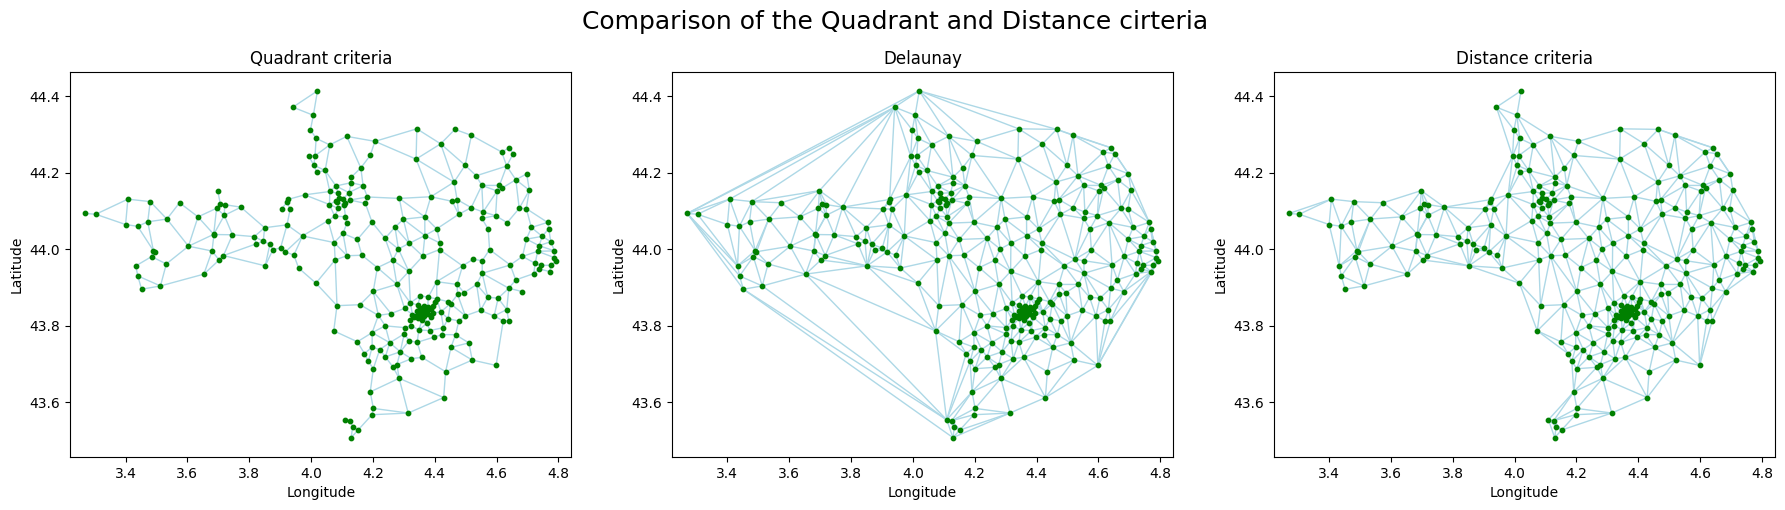
\includegraphics[width=0.9\textwidth]{images/comparaison_criteres.png}
        \caption{\label{fig:comp-crit}Evolution de la triangulation de Delaunay en fonction de critères de filtrage}
    \end{figure}
\end{frame}

\begin{frame}{Perspectives d'amélioration et travail à venir}
    \begin{block}{Améliorations}
        \begin{itemize} 
            \item Vérifier que l'algorithme du critère du quadrant donne les bons résultats;
            \item Optimisation dudit algorithme.
        \end{itemize}
    \end{block}

    \begin{block}{Travail à venir}
        \begin{itemize} 
            \item Implanter une version fonctionnelle du critère de l'angle;
            \item Se renseigner sur l'état de l'art de la théorie des graphes.
        \end{itemize}
    \end{block}
\end{frame}
}




\subsection{Brendan}
\insertsubsectionframe
\begin{frame}{Réalisation d'une interface graphique en \texttt{Python}}
    \begin{block}{Contexte}
        \begin{itemize}
            \item Beaucoup de cartes à tracer car beaucoup de paramètres ;
            \item Cartes gourmandes en ressources et pas adaptées à des notebooks \texttt{Python} ;
            \item Réalisation d'une application permettant de facilement tracer ces cartes au sein d'un navigateur web.
        \end{itemize}
    \end{block}
    
\end{frame}